\documentclass[a4j]{jsreport}

\usepackage[dvipdfmx]{graphicx}
\usepackage{multicol}
\usepackage{amsmath}
\usepackage{siunitx}
\usepackage[version=4]{mhchem}
\usepackage{url}
\usepackage{lscape}
\usepackage{multirow}
\usepackage{mathtools}


\graphicspath{{./figure/}}
\bibliographystyle{jplain}


\newcommand{\diff}{\mathrm{d}}
\DeclareSIUnit{\solventgram}{\si{\gram}\text{-solvent}}


\begin{document}

% 表紙
\begin{titlepage}
\vspace{5cm}
\centering
{\Huge トルエンの空気酸化による安息香酸の製造} \\
\vspace{2cm}
\centering
{\Large 1講座 移動現象論分野} \\
\vspace{0.5cm}
\centering
{\large 荊尾太雅 , 宮本奏汰} \\
\vspace{3cm}
\begin{table}[htbp]
    \begin{center}
        \begin{tabular}[htbp]{ll}
            \multicolumn{2}{c}{{\LARGE keyword}} \\
            {\Large 空気酸化}&{\Large Air oxidation} \\
            {\Large 気液反応}&{\Large Gas-liquid reaction} \\
            {\Large 晶析}&{\Large Crystallization} \\
            {\Large 多変数同時全体最適化}&{\Large Multi-variable simultaneous optimization} \\
            {\Large 空気}&{\Large air} \\
        \end{tabular}
    \end{center}
\end{table}
\end{titlepage}


% 目次
\pagenumbering{roman}
\setcounter{tocdepth}{2}
\tableofcontents

% 本文
\clearpage
\pagenumbering{arabic}

\chapter{緒言}
安息香酸は,主としてフェノールの原料となる他,その塩が食品や化粧品などの添加物として広く利用されている.
2014年には世界全体で48万トンが製造されており,新興国での需要から,2024年には生産量が64万トンとなると見込まれている\cite{}.
そこで,安価なトルエンを原料として用いて安息香酸を製造するプロセスを検討することにした.


\clearpage
\chapter{プロセスの概要}
\section{プロセスの概要}
本設計で対象とするのは,トルエンを空気酸化することにより安息香酸を製造するプロセスである.
プロセス全体の概略図を図\ref{プロセス全体の概略図}に示す.
\begin{figure}[htbp]
  \centering
  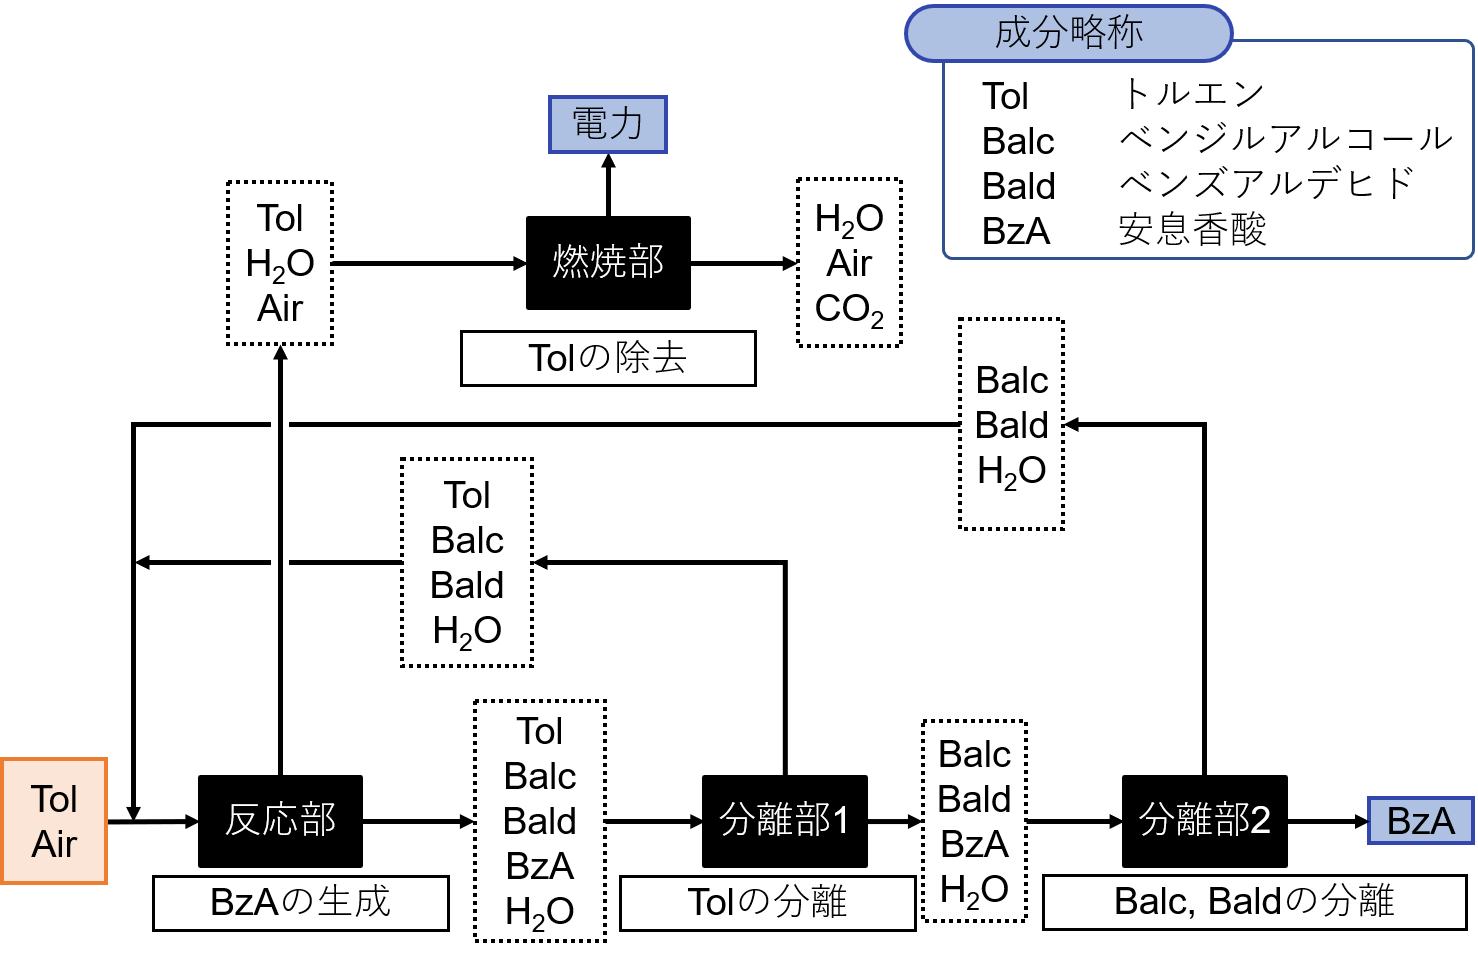
\includegraphics[scale=0.6]{processOutline.png}
  \caption{プロセス全体の概略図}
  \label{プロセス全体の概略図}
\end{figure}

\section{設計条件}
プロセスを設計するにあたり,以下の条件を設定した.
\begin{enumerate}
  \item 生産要求は,99.0wt\%以上の安息香酸を年2万トンとする.\\
  \item 工場の稼働時間は,1日24時間,年300日とする.\\
  \item 原料として,純度100\%のトルエンおよび,組成を窒素79\,mol\%酸素21\,mol\%とする空気を用いる.
           ただし,両原料は25\,\si{degreeCelsius},1\,\si{\bar}で供給されるものとする.\\
  \item 減価償却期間は8年とする.\\
  \item 圧力損失,熱損失,制御系については考慮しない.\\
  \item HYSISを用いての物性推算はUNIQUAC式によって行う.
\end{enumerate}


\clearpage
\chapter{反応部}
トルエンを空気酸化させ,安息香酸に転化させることを目的とする工程である.
反応部の概略図を図 \ref{反応部設計結果の概略図} に示す.
反応器にフィードされる液は,原料およびリサイクルによって回収された未反応トルエン,ベンジルアルコール,ベンズアルデヒド,水であり,反応器入り口において7 \si{\bar},170 \si{\degreeCelsius}に加熱および加圧され,反応器に供給される.また,反応器底部からは空気が1\,\si{\bar},25\,\si{\degreeCelsius}で供給されており,攪拌されながら反応器上方に向かう.反応器内は外部熱煤によって加熱され,7\,\si{\bar},170\,\si{\degreeCelsius}に保たれており,攪拌によって液中に溶けた酸素と未反応物質は触媒酸化反応を起こす.また,気液間物質移動により,液中のトルエンおよび水が盛んに蒸発するが,蒸発したトルエンおよび水を含む空気は反応器からコンデンサーに流入し凝縮される.凝縮したトルエンおよび水はデカンターへ送られ,密度差分離によりトルエンのみを反応器に還流し,水はパージする.また,凝縮しなかったトルエンは,環境安全上の理由からそのまま排出することはできないので,濃度を減少させるために燃焼部へと送られる.反応器からの流出液は次の工程である分離部1へと送られる.
\begin{figure}[htbp]
  \centering
  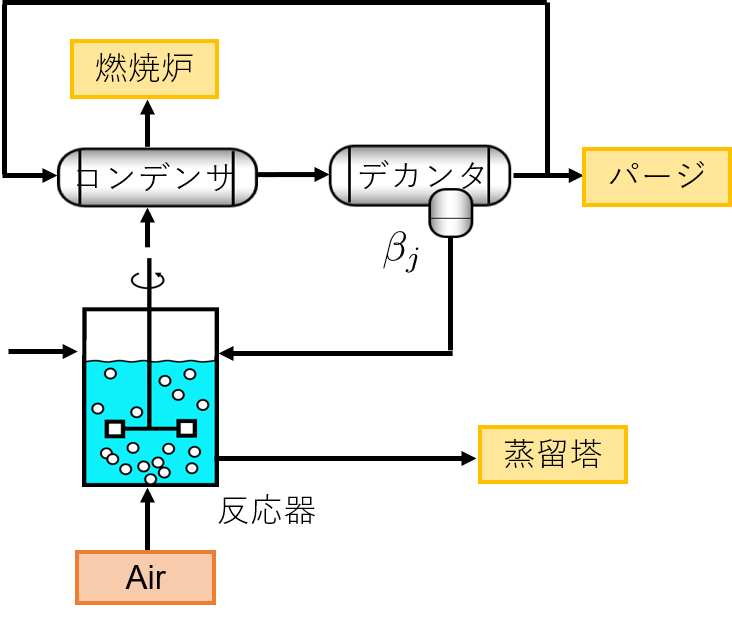
\includegraphics[scale=0.7]{ReactionSection.png}
  \caption{反応部概略図}
  \label{反応部設計結果の概略図}
\end{figure}

\section{反応機構}
今回用いた反応は以下の4つである.トルエンは経路によらず最終的に安息香酸へと転化する.
\begin{center}
\begin{tabular}{lcrlll}
  \ce{Tol} & + & \ce{O2} & \ce{-> Bald + H2O} & $r_1 = k_1 \cdot C_\text{Tol}$ & $\varDelta _\mathrm{r} H_1 = -385.23$ \, \si{\kilo \joule \per \mole} \\
  \ce{Tol} & + & 1/2 \ce{O2} & \ce{-> Balc} & $r_2 = k_2 \cdot C_\text{Tol}$ & $\varDelta _\mathrm{r} H_2 = -167.30$ \, \si{\kilo \joule \per \mole} \\
  \ce{Balc} & + & 1/2 \ce{O2} & \ce{-> Bald + H2O} & $r_4 = k_3 \cdot C_\text{Balc}$ & $\varDelta _\mathrm{r} H_3 = -317.30$ \, \si{\kilo \joule \per \mole} \\
  \ce{Bald} & + & 1/2 \ce{O2} & \ce{-> BzA} & $r_3 = k_4 \cdot C_\text{Bald}$ & $\varDelta _\mathrm{r} H_4 = -298.20$ \, \si{\kilo \joule \per \mole}
\end{tabular}
\end{center}

ただし,トルエンをTol,ベンジルアルコールをBalc,ベンズアルデヒドをBald,安息香酸をBzAと表記している.これらの反応は全て酸化反応であり,触媒には,酸化剤であるモリブデン酸マンガン\ce{MnMoO4}を用いることとした.これらの反応の反応速度定数は,表\ref{反応速度定数}のようである\cite{}.
\begin{table}[htbp]
  \centering
  \label{反応速度定数}
  \caption{各反応式の反応速度定数}
  \begin{tabular}{ccccc}
    \hline
    & $k_1$ & $k_2$ & $k_3$ & $k_4$ \\
    \hline
    $\ln A_j \, [\si{-}]$ & 17.93 & 20.63 & 15.40 & 19.70 \\
    $E_j \, [\si{\kilo \joule \per \mole}]$ & 69.53 & 81.39 & 56.99 & 71.44 \\
    \hline
  \end{tabular}
\end{table}

また,酸化反応が激しい場合には燃焼反応によって二酸化炭素まで転化するので,反応器における反応率が高い場合には考慮する必要があるが,
今回の設計結果では単通反応率が0.265と低かったため,燃焼反応は無視できると考えた.

\section{反応器選定}
流通式の気液反応器の種類には,拡散速度に対して不利な順に,気泡塔,気液攪拌槽,充填塔などがある.
反応器を選定するにあたり,最大反応速度と最大拡散速度の比を表す八田数を概算し,八田数が0.1より小さいなら気泡塔,5より大きければ充填塔,中間域ならば気液攪拌槽を選択することとした\cite{化工便覧}.
今回は気液攪拌槽型反応器を選択した.実際のプロセスでは気泡塔も選択される.

反応器内攪拌には6枚羽根タービン翼を用い,空気流入による冷却作用が大きいため,ジャケットを取り付け,ジャケット内部に熱媒を流している.
また,空気を反応器内に送るスパージャー直径は反応器直径の1/3とした.\\

八田数の定義式
\begin{equation}
    \gamma = \frac{\text{(最大反応速度)}}{\text{(最大拡散速度)}} = \frac{(C_\mathrm{B} k D_\mathrm{B})^{1/2}}{k_\mathrm{L}}
\end{equation}

\section{設計方程式}
両相の滞留時間の大きさが十分異なると考えられることから,
液相は完全混合状態として,気相は鉛直方向に向かう押し出し流れと仮定できると判断した.
設計時に用いた仮定は以下のようである.
\begin{itemize}
    \item[-] 気相は水平方向に一様な濃度分布を持つ.
    \item[-] 気相側境膜抵抗は無視できる
    \item[-] 液相は完全混合状態である.
    \item[-] 窒素,酸素はヘンリー則に従い,その他の物質はラウール則に従う.
\end{itemize}
以上の仮定および,蒸発油分を還流する機構を含めて,設計方程式\eqref{液相物質収支式},\eqref{気相物質収支式},\eqref{熱収支式}を立式した.
\begin{equation}
    \label{液相物質収支式}
    0 = F^\text{in}_{\text{liq},j} - F^\text{out}_{\text{liq},j} - (1 - \beta_j) k_\mathrm{L} a \int^{V_\text{tot}}_0(C_j - C^\text{sat}_j) \diff V + r_j V_\mathrm{L}
\end{equation}
\begin{equation}
    \label{気相物質収支式}
    \frac{\diff F_{\text{gas},j}}{\diff V} = k_\mathrm{L} a (C_j - C^\text{sat}_j)
\end{equation}
\begin{equation}
    \label{熱収支式}
    \sum_jF_{j,\mathrm{in}}H_{j,\mathrm{in}}-\sum_jF_{j,\text{out}}H_{j,\text{out}} = UA(T_\mathrm{s}-T)
\end{equation}

解析方法としては,まず油分を全還流として近似的に各液相中濃度を決定した.そして,トルエンおよび,酸素,窒素について濃度を仮定した後に,
気相の物質収支式をRunge-kutta法によって計算し,各蒸発量が収支式と一致する濃度を求めた.
また,物質移動容量係数が十分大きいと判断し,最適化中の解析に用いる場合には,気相は迅速に平衡状態へ達すると仮定した.

\section{物質移動容量係数の推算}
物質移動容量係数は,反応装置形状,反応器内部流体の様々な物性,流れの状態に依存する.攪拌槽型反応器に対し,物質移動容量係数の推算に用いた各相関式を記す.

\noindent 液相側物質移動係数の相関式\cite{化工便覧}\\
% \item[] 小気泡の場合
% \begin{equation}
%     k_\mathrm{L} = 0.31Sc_\mathrm{L}^{-2/3}(g \varDelta \rho \mu_\mathrm{L}/\rho_\mathrm{L}^2)^{1/3}
% \end{equation}
% \item[] 大気泡の場合
% \begin{equation}
%     k_\mathrm{L} = 0.42Sc_\mathrm{L}^{-1/2}(g \varDelta \rho \mu_\mathrm{L}/\rho_\mathrm{L}^2)^{1/3}
% \end{equation}
\begin{align}
  \text{小気泡の場合 : } &k_\mathrm{L} = 0.31Sc_\mathrm{L}^{-2/3}(g \varDelta \rho \mu_\mathrm{L}/\rho_\mathrm{L}^2)^{1/3} \\
  \text{大気泡の場合 : } &k_\mathrm{L} = 0.42Sc_\mathrm{L}^{-1/2}(g \varDelta \rho \mu_\mathrm{L}/\rho_\mathrm{L}^2)^{1/3}
\end{align}

\noindent 比表面積の相関式\cite{化工便覧}
\begin{equation}
    a = 1.44 \left( \frac{P_\mathrm{V}^{0.4} \rho_\mathrm{L}^{0.2} }{ \sigma^{0.6}} \right) \left( \frac{u_\mathrm{G}}{u_\mathrm{t}} \right)^{0.5} \left( \frac{P_\mathrm{T}}{P_\mathrm{G}} \right) \left( \frac{\rho_\mathrm{G}}{\rho_\mathrm{a}} \right)^{0.16}
\end{equation}

上記の2式を利用するために用いた相関式を以下に記す.

\noindent ガスホールドアップの相関式\cite{化工便覧}
\begin{equation}
    \varepsilon_{{\mathrm G}} = \left( \frac{u_{{\mathrm G}}\varepsilon_{{\mathrm G}}}{u_{{\mathrm t}}} \right) + 0.000216 \times \left( \frac{P_\mathrm{V}^{0.4} \rho_\mathrm{L}^{0.2} }{ \sigma^{0.6}} \right) \left( \frac{u_\mathrm{G}}{u_\mathrm{t}} \right)^{0.5} \left( \frac{P_\mathrm{T}}{P_\mathrm{G}} \right) \left( \frac{\rho_\mathrm{G}}{\rho_\mathrm{a}} \right)^{0.16}
\end{equation}

\noindent 気泡の体積平均径の相関式\cite{化工便覧}
\begin{equation}
    d_\mathrm{vs} = 4.15 \left( \frac{\sigma^{0.6}}{P_\mathrm{V}^{0.4} \rho_\mathrm{L}^{0.2}} \right) \left( \frac{P_\mathrm{G}}{P_\mathrm{T}} \right) \left( \frac{\rho_\mathrm{a}}{\rho_\mathrm{G}} \right) ^{0.16} \varepsilon_\mathrm{G}^{0.5} + 0.0009
\end{equation}

\noindent 気泡の終末速度の相関式\cite{化工便覧}
\begin{equation}
    u_\mathrm{t} = \left( \frac{4\varDelta \rho g d_\mathrm{vs}}{3C_\mathrm{D} \rho_\mathrm{L}} \right)^{0.5}
\end{equation}

さらに,上記の相関式を利用するために用いた物性値の推算式,および変数の定義式などの諸式を以下に記す.

\noindent 抗力係数の相関式\cite{19952357}
\begin{equation}
    C_\mathrm{D} = \max \left[ \frac{24}{Re}(1+0.15Re^{0.687}), \, \frac{8}{3} \frac{Eo}{Eo+4} \right]
\end{equation}
拡散係数の推算\\
wilke-changの式\cite{化工便覧}
\begin{equation}
    D_{12} = \frac{2.946\times 10^{-11}(\beta M_{\mathrm{r,2}})^{1/2} T} {\mu_2 V_{\mathrm{b},1}^{0.6}}
\end{equation}
Einstin-Stokesの式\cite{実験テキスト}
\begin{equation}
    \frac{D \mu}{T} = \text{const}
\end{equation}

\noindent 界面張力の推算

\noindent 界面張力の温度依存性に関する相関式\cite{化工便覧}
\begin{equation}
    \sigma \propto \{ 1-(T/T_\mathrm{c}) \}^n
\end{equation}

\noindent 気泡レイノルズ数の定義式\cite{19952357}
\begin{equation}
    Re = \frac{\rho_\mathrm{L}u_\mathrm{t} d_\mathrm{vs}}{\mu_\mathrm{L}}
\end{equation}
\noindent エトベス数の定義式\cite{19952357}
\begin{equation}
    Eo = \frac{g \varDelta \rho d_\mathrm{vs}^2}{\sigma}
\end{equation}

また,参考文献\cite{化工便覧}からトルエンの標準沸点における分子容積を\si{\cubic \centi \metre \per \mole}とし,
参考文献\cite{界面張力}からトルエンの界面張力$\sigma=0.81 \,\si{\newton \per \metre \squared}$とし,
参考文献\cite{TPP}から会合度を1とした.

以上の諸式を用いて物質移動容量係数を推算した.結果は反応器設計結果で示す.

\section{反応器設計結果}
最終結果における反応器の詳細を表\ref{反応器設計結果の表}に示す.
\begin{table}[htbp]
  \centering
  \caption{反応器設計結果}
  \label{反応器設計結果の表}
  \begin{tabular}{cc}
    \hline
    項目 & 値 \\
    \hline
    反応器内圧力 \, [\si{bar}] & 7.00 \\
    反応器内温度 \, [\si{\degreeCelsius}] & 170 \\
    反応器体積 \, [\si{\cubic \metre}] & 14.6 \\
    気液総体積 \, [\si{\cubic \metre}] & 8.25 \\
    単通販能率 \, [\si{-}] &0.265\\
    ガスホールドアップ \, [\si{-}] & 0.115  \\
    液平均滞留時間 \, [\si{\hour}] & 0.478  \\
    物質移動容量係数 \, [\si{\per \second}] & 0.470  \\
    液相物質移動係数 \, [\si{\metre \per \second}] & 0.00172 \\
    比界面積 \, [\si{\per \metre}] & 273 \\
    反応器空間率 \, [\si{-}] & 0.435 \\
    総攪拌動力 \, [\si{\kilo \watt}] & 8.25 \\
    気泡体積平均径 \, [\si{\milli \metre}] & 2.53 \\
    エトベス数 \, [\si{-}] & 1480 \\
    気泡レイノルズ数 \, [\si{-}] & 1170 \\
    \hline
  \end{tabular}
\end{table}

\section{反応部設計結果}
最適化後の最終結果における反応部の物質収支を図\ref{反応部設計結果の図}中に示す.最適化方法については最適化の章で述べる.
\begin{figure}[htbp]
  \centering
  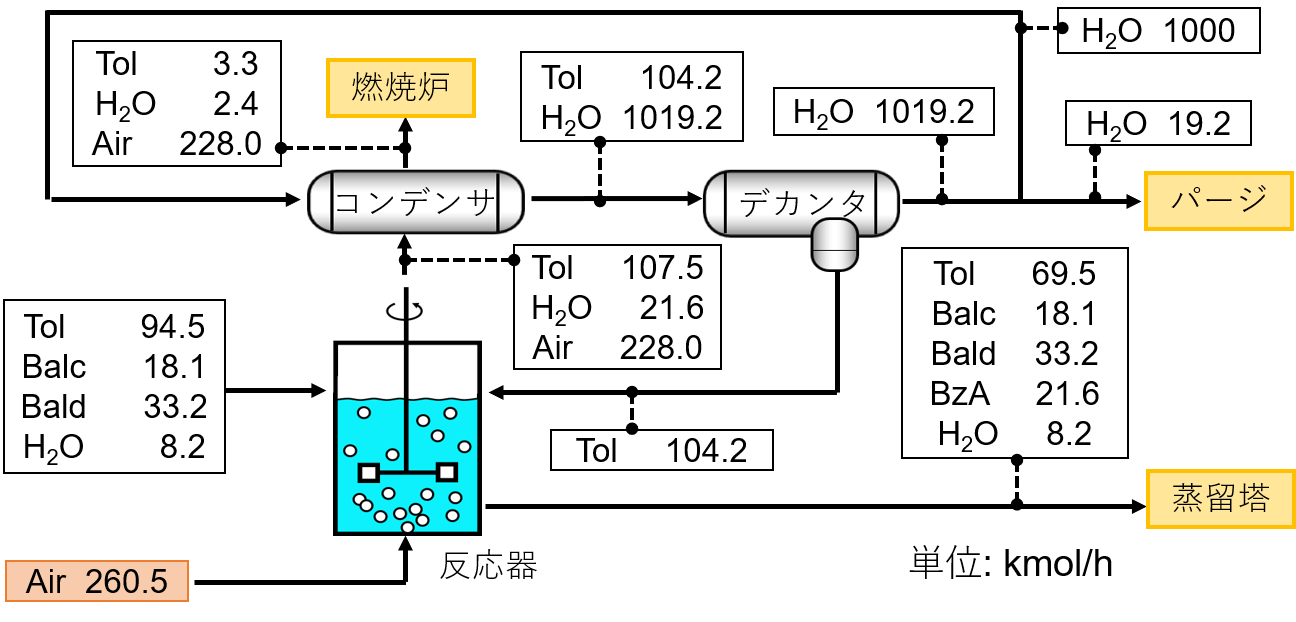
\includegraphics[scale=0.7]{ReactionSectionConclusion.png}
  \caption{反応部設計結果}
  \label{反応部設計結果の図}
\end{figure}


\clearpage
\chapter{分離部1}
\section{蒸留塔設計}
未反応トルエンのうち99\,\%以上を回収することを目的とした.
設計条件として,蒸留塔段数を10段,蒸留塔供給段は6段,還流比を1.0とした.

蒸留塔圧力を変更し,全体の利益を最大とする点について探索を行った.
反応器流出液圧力が7\,\si{\bar}であるため,最適な圧力であることが予想される.
蒸留塔の圧力を変化させ,人件費を除く全体の利益を評価関数としてプロットした
図\ref{蒸留塔圧力最適化}から,確かに7\,\si{\bar}で全体の利益が最大化されることを確認した.
\begin{figure}[htbp]
  \centering
  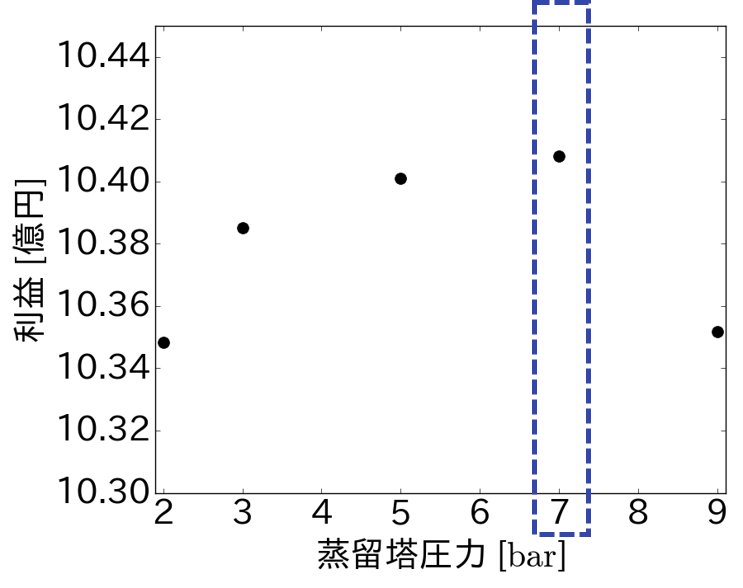
\includegraphics[scale=0.7]{DistillationPressue.png}
  \caption{蒸留塔圧力最適化}
  \label{蒸留塔圧力最適化}
\end{figure}

設計結果を表\ref{蒸留塔設計結果}に記す.
\begin{table}[htbp]
  \label{蒸留塔設計結果}
  \caption{蒸留塔設計結果}
  \centering
  \begin{tabular}{cc}
      \hline
      項目 & 値 \\
      \hline
      塔径 \, [\si{\metre}] & 1.0 \\
      塔高 \, [\si{\metre}] & 6.1 \\
      塔内圧力 \, [\si{\bar}] &7 \\
      コンデンサ内温度 \, [\si{\degreeCelsius}] & 232 \\
      リボイラー内温度 \, [\si{\degreeCelsius}] & 316 \\
      \hline
  \end{tabular}
\end{table}

\section{分離部1設計結果}
最適化後の最終結果における分離部1の流量関係を図\ref{分離部1設計結果の図}中に示す.
\begin{figure}[htbp]
  \centering
  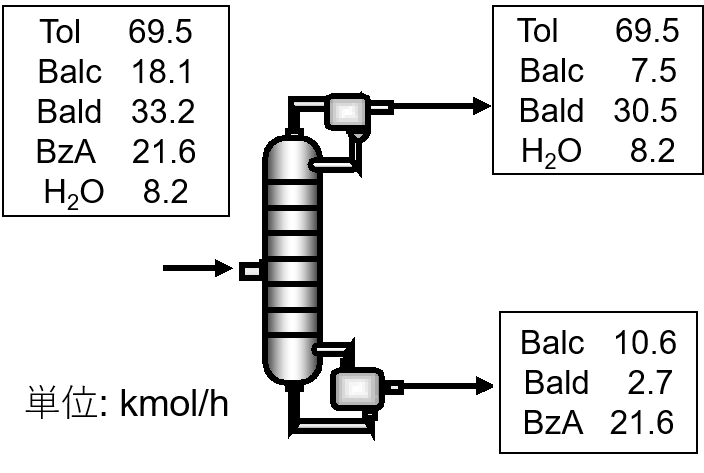
\includegraphics[scale=0.7]{Separation1Conclusion.png}
  \caption{分離部1設計結果}
  \label{分離部1設計結果の図}
\end{figure}


\clearpage
\chapter{分離部2}
\section{晶析器選定}
溶解度の温度依存性が大きいことと,目的とする結晶生産量が大きいことから,
連続式攪拌槽型反応装置を選定した.

\noindent 溶解度の温度依存性の相関式
\begin{equation}
    C^*=2.03\times 10^{-5}T^4 +2.03^{-5}\times T^4 + 2.97\times 10^{-4}T^3 + 4.70\times 10^{-2}T^2 + 1.43T + 24.71
\end{equation}
ただし,温度$T \, [\si{\degreeCelsius}]$,溶解度$C^* \, [\si{\gram \per \kilo \solventgram}]$
\begin{figure}[htbp]
  \centering
  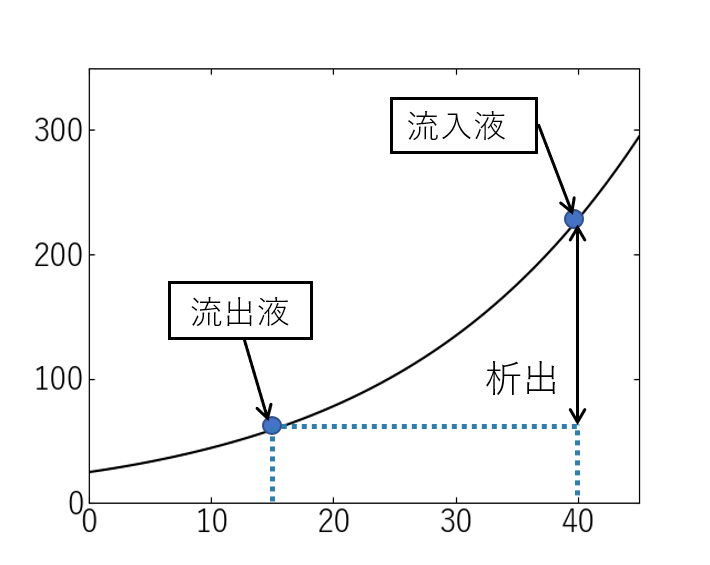
\includegraphics[scale=0.7]{BzAsolvent.png}
  \caption{溶解度の温度依存性}
  \label{溶解度の温度依存性}
\end{figure}

\section{設計方程式}
以下の仮定を用いた.
\begin{itemize}
    \setlength{\parskip}{0pt}
    \setlength{\itemsep}{2pt}
    \item[-] 結晶表面拡散は迅速に行われる.
    \item[-] 晶析器内は完全混合状態である.
    \item[-] 二次核発生の影響は無視する.
\end{itemize}

参考文献\cite{晶析}により,以下の実験式および理論式を用いて設計を行った.\\
一次核発生速度
\begin{equation}
    B^0 = k_\mathrm{b} M_\mathrm{T}^j \Delta C^b
\end{equation}
結晶成長速度
\begin{equation}
    G = k_\mathrm{g}\Delta C^g
\end{equation}
結晶成長速度定数
\begin{equation}
    k_\mathrm{g} = k_\mathrm{g0} \exp \left( -\frac{E_\mathrm{g}}{RT} \right)
\end{equation}
個数収支式
\begin{equation}
    n=n^0 \exp \left( -\frac{L}{G\tau} \right)
\end{equation}
懸濁密度
\begin{equation}
    M_\mathrm{T} = c_0-c = 6k_\mathrm{v} \rho_\mathrm{c} n^0 (G\tau)^4
\end{equation}
各パラメータは以下の通りである.
\begin{align*}
    &k_\mathrm{g0} = 1.06\times10^7 \, \si{(\micro \meter)(\gram / \solventgram)^{\textit{-g}}} \\
    &B^{\mathrm{0}} = 40.05 \, \si{\kilo \joule \per \mole} \\
    &k_\mathrm{b} = 9.16 \times 10^{12} \, \si{(\# / \cubic \meter \second) (\gram / \milli \liter)^{\textit{-j}} (\gram / \solventgram)^{\textit{-b}}} \\
    &g = 0.44 \\
    &j = 1.78 \\
    &b = 1.2 \\
    &k_\mathrm{v} = 0.1 \\
    &\rho_\mathrm{c} = 1.32 \, \si{\gram \per \centi \metre \cubed}
\end{align*}

\section{晶析器設計結果}
最適化の結果によって得られた晶析器の設計結果を表\ref{晶析器設計結果}に記す.
\begin{table}[htbp]
  \centering
  \caption{晶析器設計結果}
  \label{晶析器設計結果}
  \begin{tabular}{cc}
    \hline
    項目 & 値 \\
    \hline
    晶析器体積 \, [\si{\cubic \metre}] &7.16 \\
    晶析器液体積 \, [\si{\cubic \metre}] &3.58 \\
    晶析器フィード液温 \, [\si{\degreeCelsius}] & 40.0 \\
    晶析器内温度 \, [\si{\degreeCelsius}] &13.3 \\
    晶析器内圧力 \, [\si{bar}] &1.00 \\
    滞留時間 \, [\si{min}] &9.71 \\
    単通結晶収率 \, [\si{-}] &0.690 \\
    結晶化可能量基準収率 \, [\si{-}] &0.902 \\
    結晶の体積平均径 \, [\si{\micro \metre}] &3.41 \\
    \hline
  \end{tabular}
\end{table}

\section{抽出塔設計}
十分に塔内へ液を滞留させることによって安息香酸を水中に飽和させることを目的とした.
十分なデータを得られなかったため,2時間の装置内滞留によって安息香酸がトルエン溶媒中に飽和し,
その他ベンジルアルコール,ベンズアルデヒドの溶解度については無視できると仮定した.

\section{分離部2設計結果}
分離部2のみの流量関係を簡易的に図\ref{分離部2設計結果}中に示す.
蒸留塔から送られてきた油液は冷却され,抽出塔内に供給される.晶析器で用いた安息香酸水溶液を加熱し,溶解度を上昇させて抽出塔内に供給する.
抽出塔内では安息香酸が水中に溶解し,ベンジルアルコール,ベンズアルデヒドおよび触媒は溶解せずに回収され,反応部へ送られる.安息香酸水溶液を晶析器に供給し,製品結晶を得ている.

\begin{figure}[htbp]
  \centering
  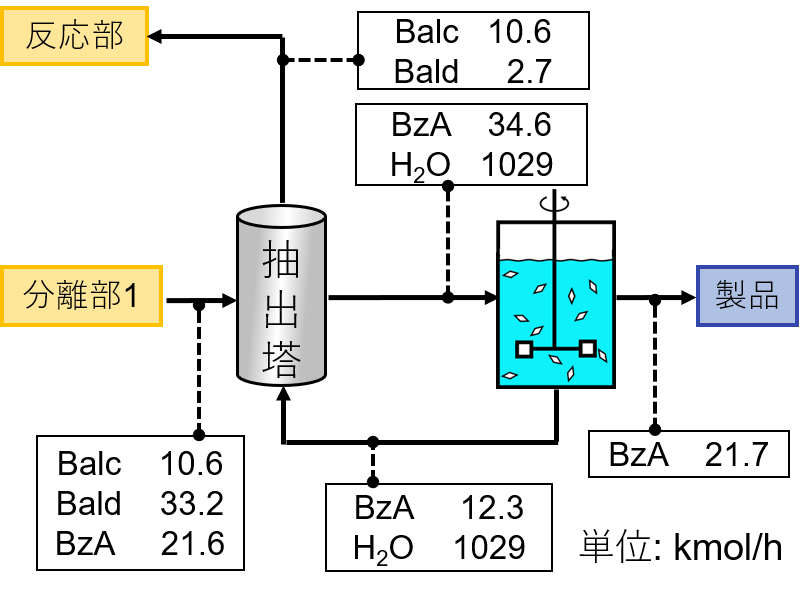
\includegraphics[scale=0.7]{Separion2Conclusion.png}
  \caption{分離部2設計結果}
  \label{分離部2設計結果}
\end{figure}


\clearpage
\chapter{燃焼部}
トルエンは人体に有害な物質であり,吸引によって神経系などに深刻な被害を与えることもある.
東京都の条例には排出基準が厳しく定められており,この基準を満たすため,反応部のコンデンサーで凝縮しなかったトルエンを燃焼させることでその濃度を減じる.
燃焼炉内ではトルエンが完全燃焼し,二酸化炭素および水へ転化すると仮定し,量論的に燃焼に必要な量と等量の酸素を供給して燃焼炉へと送るものとした.
燃焼熱は熱媒の作成に使用され,足りない分は燃料を投入して賄っているものと考えた.

\clearpage
\chapter{最適化}
\section{方法}
最適化を行うにあたり,最適化変数として以下の3つを選択した.
\begin{itemize}
  \item 反応器体積
  \item 晶析器体積
  \item 晶析器温度
\end{itemize}

これらの変数を選択した理由を述べる.反応器体積が大きいとき,反応器の装置コストは大きくなる.一方で,反応器出口から排出される未反応トルエンの量が減るため,蒸留塔のリボイラーで必要な熱量が減少し,熱煤のコストは減少する.反応器体積が小さいときは,反応器の装置コストは小さくなるが,熱煤のコストは大きくなる.晶析器体積が大きいとき,晶析器の装置コストは大きくなる.しかし,晶析する安息香酸の量が増えるため,リサイクルに回る安息香酸の量が少なくなり,それを保持するための純水の量が減少し,純水の費用は抑えられる.晶析器の体積が小さいときは,逆になる.晶析器温度が低い時,必要な外部冷媒の温度が低くなるため,冷媒の単価は高くなる.しかし,晶析する安息香酸の量が大きくなるため,リサイクルに回る安息香酸の量が小さくなり,必要な純水の量が減るため,純水を冷やすために用いている冷媒の量は小さく抑えられる.晶析器温度が高いときは,冷媒の単価は安くなるが,冷媒の必要量が大きくなる.このように,最適化変数に選択した変数は,その大小によって,なんらかのトレードオフの関係を生じる.そのため,これらの変数の値を変化させることで,利益が最大となる最適点を探索することが可能であると考えた.

次に,最適化の具体的な手法について述べる.プロセスを最適化するにあたり,3つの最適化変数変数全てを同時に最適化することを考えた.そこで,反応器体積は,$13.5 \sim 16.0 \, \si{\cubic \metre}$の範囲で6点,晶析器体積は,$6 \sim 12 \, \si{\cubic \metre}$の範囲で13点,晶析器温度は,$5.0 \sim 20.0 \, \si{\degreeCelsius}$の範囲で16点,計1248点のデータを取った.そして,それぞれのデータについてフィッティングを行った後に,それぞれの範囲を100当分し,データの個数を$100 \times 100 \times 100$点に増やした.それらのデータを用いて,横軸に晶析器温度,縦軸に晶析器体積を設定し,反応器体積の値を逐次的に変化させることで,100枚のヒートマップを作成した.ヒートマップが表す値は,
\begin{equation}
  \text{P.I.} = \text{(売上)} - \text{(原料コスト)} - \text{(装置コスト)} -\text{(用役コスト)}
\end{equation}
で表される評価関数の値とした.また,各ヒートマップ上で,評価関数の値が最大となる点をプロットした.さらに,そのプロットがどのように変化するかを見るために,横軸に反応器体積,縦軸に評価関数の値を取り,折れ線グラフを作成した.

\section{最適化結果}
評価関数の値が最大となった点での,ヒートマップおよび,評価関数の最大値の変化を表したグラフは図\ref{最適化結果}のようになった.また,作成したgifはgithubにアップしているので,興味のある方はご覧ください(\url{https://github.com/miyamo-sou/processdesign}).最適点での反応器体積は14.69\, \si{\cubic \metre},晶析器体積は7.16\, \si{\cubic \metre},晶析器温度は13.3\, \si{\degreeCelsius}となった.また,その時の評価関数の値は10.35億円となった.
\begin{figure}[htbp]
  \centering
  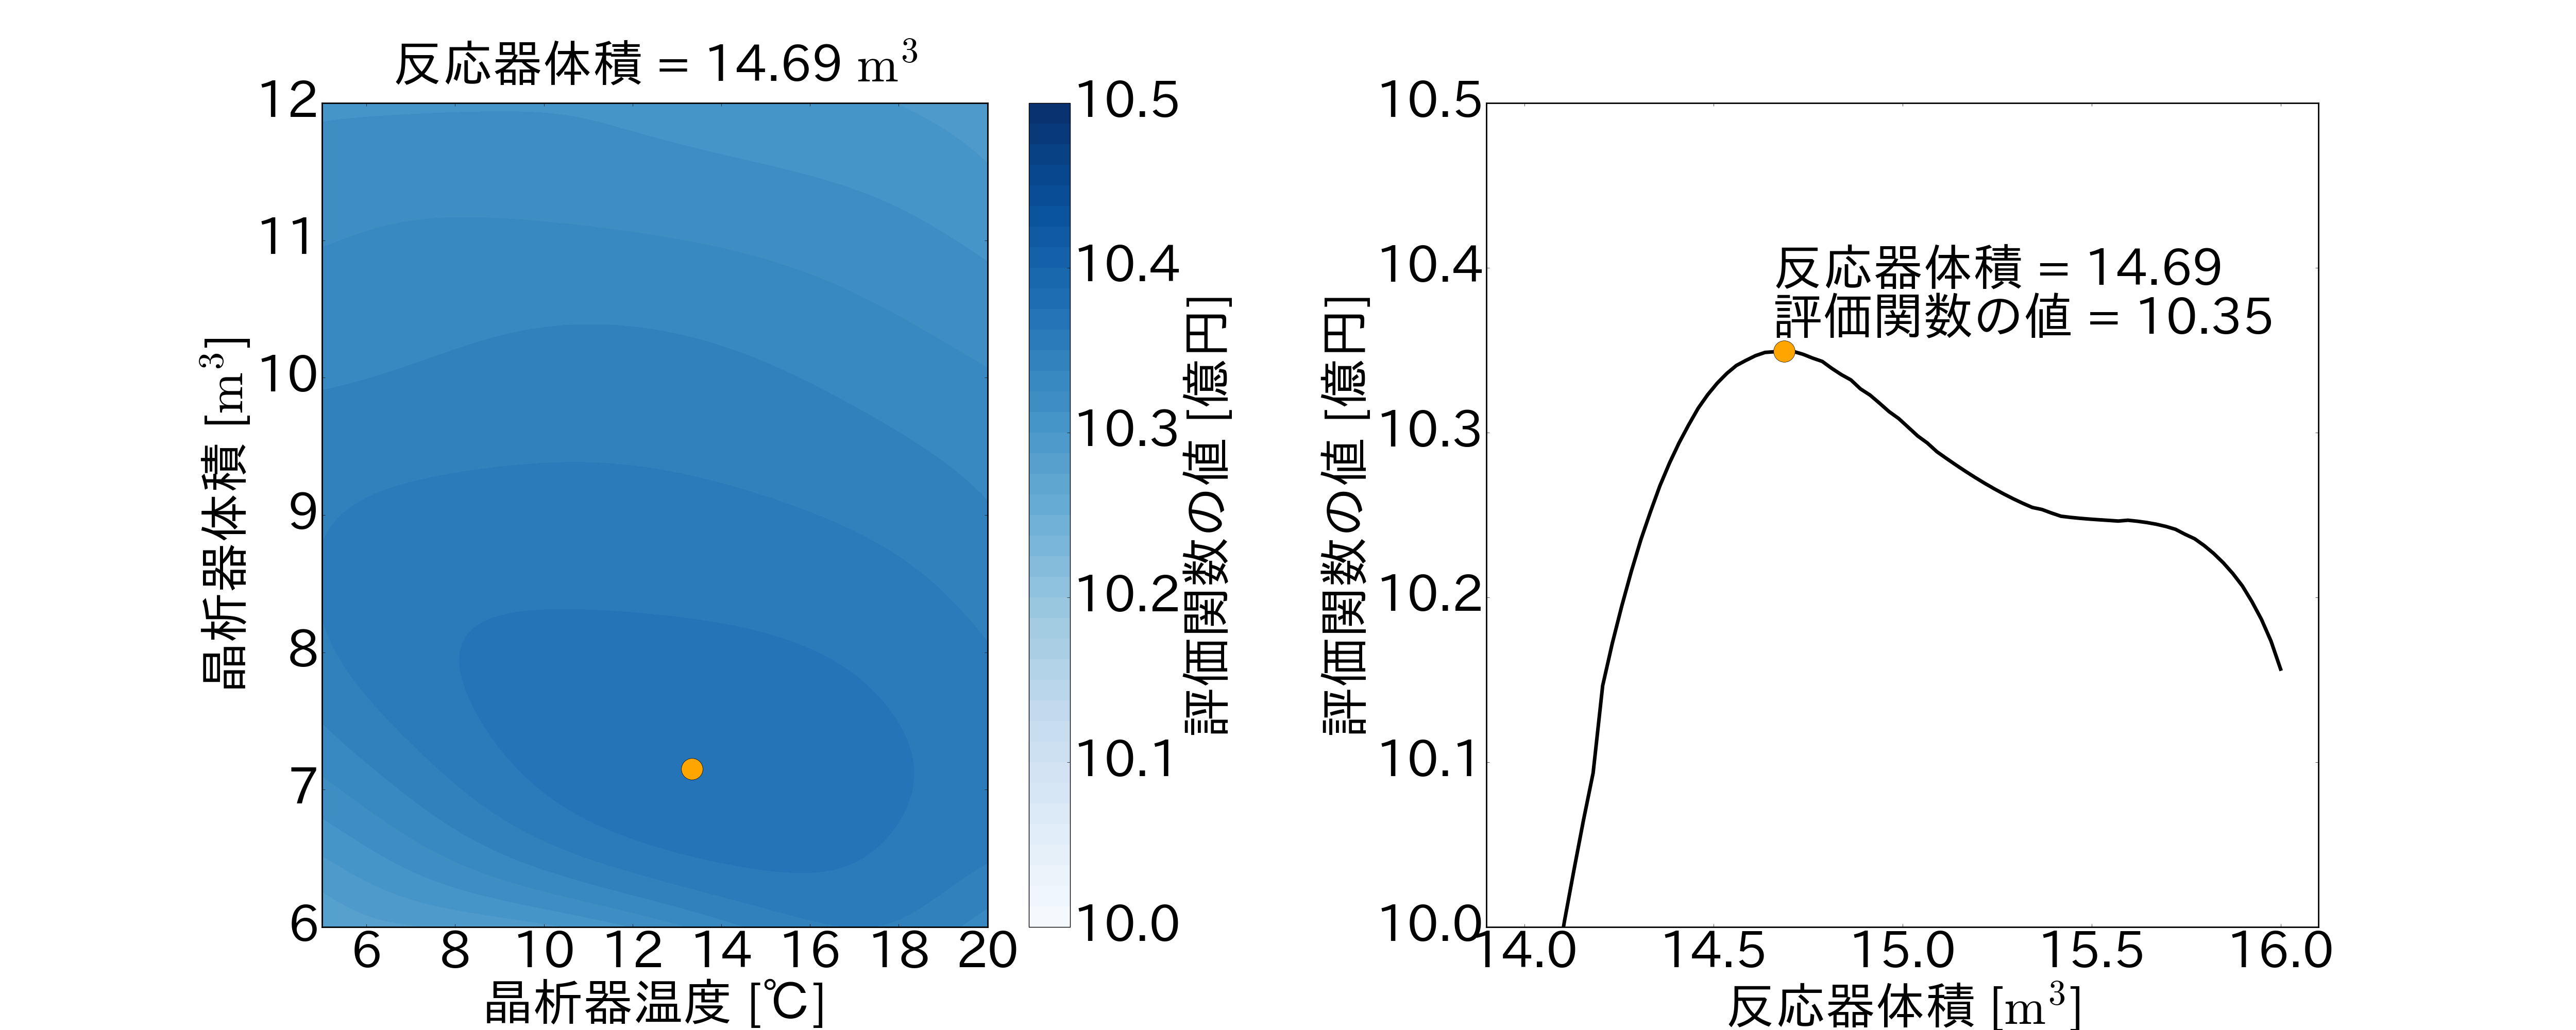
\includegraphics[scale=0.1]{snapshot.png}
  \caption{評価関数の値が最大となる点でのヒートマップと最適点の推移}
  \label{最適化結果}
\end{figure}

このよに,評価関数は大きなピークが存在する形になっていることが分かる.これは,最適化方法のセクションでも述べたが,反応器体積,晶析器体積,晶析器温度を変化させると,装置費と用役費がトレードオフの関係となって,コストが変化する.そのため,このようにピークが生じたと考えられる.


\clearpage
\chapter{物質収支 $\cdot$ 熱収支}
全体のフロー図は図\ref{フロー図}のようになった.
\begin{figure}[htbp]
  \centering
  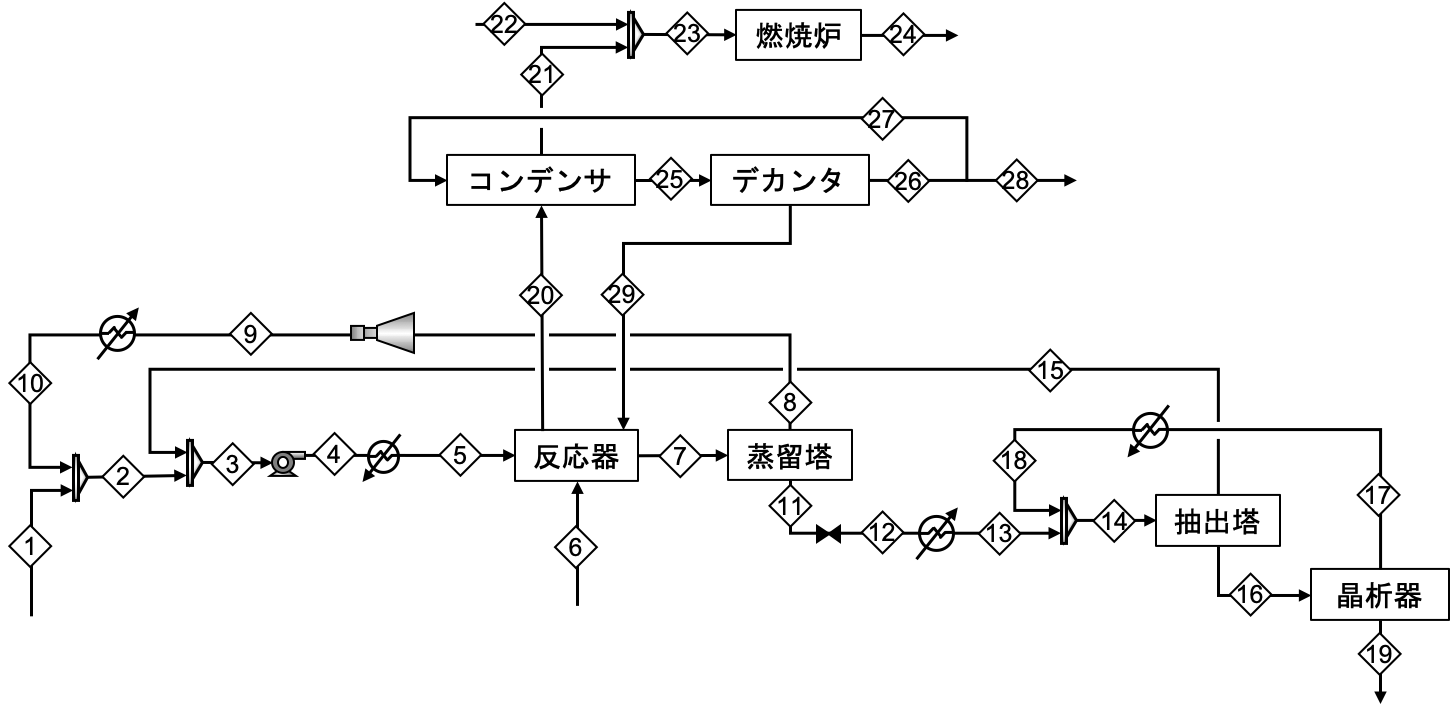
\includegraphics[scale=0.6]{mat_flow.png}
  \caption{フロー図}
  \label{フロー図}
\end{figure}

また,フロー図に記載されているフローの組成および温度,圧力は表\ref{流量関係1},\ref{流量関係2},\ref{流量関係3}のようになった.
\begin{table}[htbp]
  \centering
  \caption{流量関係}
  \label{流量関係1}
  \begin{tabular}{ccccccccccccccc}
    \hline
    [\si{\kilo \mole \per \hour}] & 1 & 2 & 3 & 4 & 5 & 6 & 7 & 8 & 9 & 10 \\
    \hline
    トルエン & 25 & 94.5 & 94.5 & 94.5 & 94.5 & 0 & 69.5 & 69.5 & 69.5 & 69.5 \\
    ベンジルアルコール & 0 & 7.5 & 18.1 & 18.1 & 18.1 & 0 & 18.1 & 7.5 & 7.5 & 7.5 \\
    ベンズアルデヒド & 0 & 30.5 & 33.2 & 33.2 & 33.2 & 0 & 33.2 & 30.5 & 30.5 & 30.5 \\
    安息香酸 & 0 & 0 & 0 & 0 & 0 & 0 & 21.6 & 0 & 0 & 0 \\
    水 & 0 & 8.2 & 8.2 & 8.2 & 8.2 & 0 & 8.2 & 8.2 & 8.2 & 8.2 \\
    空気 & 0 & 0 & 0 & 0 & 0 & 260.5 & 0 & 0 & 0 & 0 \\
    二酸化炭素 & 0 & 0 & 0 & 0 & 0 & 0 & 0 & 0 & 0 & 0 \\
    \hline
    合計 & 25 & 140.7 & 154 & 154 & 154 & 260.5 & 150.6 & 115.7 & 115.7 & 115.7 \\
    \hline
    温度 \, [\si{\degreeCelsius}] & 25 & 79.9 & 75.56 & 76.04 & 170 & 25 & 170 & 231.5 & 194.8 & 90.88 \\
    圧力 \, [\si{\bar}] & 1 & 1 & 1 & 7 & 7 & 1 & 7 & 7 & 1 & 1 \\
    \hline
  \end{tabular}
\end{table}

\begin{table}[htbp]
  \centering
  \caption{流量関係}
  \label{流量関係2}
  \begin{tabular}{ccccccccccccccc}
    \hline
    [\si{\kilo \mole \per \hour}] & 11 & 12 & 13 & 14 & 15 & 16 & 17 & 18 & 19 & 20 \\
    \hline
    トルエン & 0 & 0 & 0 & 0 & 0 & 0 & 0 & 0 & 0 & 107.5 \\
    ベンジルアルコール & 10.6 & 10.6 & 10.6 & 10.6 & 10.6 & 0 & 0 & 0 & 0 & 0 \\
    ベンズアルデヒド & 2.7 & 2.7 & 2.7 & 2.7 & 2.7 & 0 & 0 & 0 & 0 & 0 \\
    安息香酸 & 21.6 & 21.6 & 21.6 & 34.6 & 0 & 34.6 & 13 & 13 & 21.6 & 0 \\
    水 & 0 & 0 & 0 & 1029 & 0 & 1029 & 1029 & 1029 & 0 & 21.6 \\
    空気 & 0 & 0 & 0 & 0 & 0 & 0 & 0 & 0 & 0 & 228 \\
    二酸化炭素 & 0 & 0 & 0 & 0 & 0 & 0 & 0 & 0 & 0 & 0 \\
    \hline
    合計 & 34.9 & 34.9 & 34.9 & 1076.9 & 13.3 & 1063.6 & 1042 & 1042 & 21.6 & 357.1 \\
    \hline
    温度 \, [\si{\degreeCelsius}] & 315.6 & 230.9 & 25 & 25 & 40 & 40 & 13.3 & 40 & 13.3 & 25 \\
    圧力 \, [\si{\bar}] & 7 & 1 & 1 & 1 & 1 & 1 & 1 & 1 & 1 & 1 \\
    \hline
  \end{tabular}
\end{table}

\begin{table}[htbp]
  \caption{流量関係}
  \label{流量関係3}
  \centering
  \begin{tabular}{ccccccccccccccc}
    \hline
    [\si{\kilo \mole \per \hour}] & 21 & 22 & 23 & 24 & 25 & 26 & 27 & 28 &  &  \\
    \hline
    トルエン & 3.4 & 0 & 3.4 & 0 & 104.1 & 0 & 0 & 0 &  &  \\
    ベンジルアルコール & 0 & 0 & 0 & 0 & 0 & 0 & 0 & 0 &  &  \\
    ベンズアルデヒド & 0 & 0 & 0 & 0 & 0 & 0 & 0 & 0 &  &  \\
    安息香酸 & 0 & 0 & 0 & 0 & 0 & 0 & 0 & 0 &  &  \\
    水 & 2.4 & 0 & 2.4 & 15.8 & 0 & 0 & 0 & 0 &  &  \\
    空気 & 228 & 39.4 & 267.4 & 237.8 & 1019.2 & 1019.2 & 1000 & 19.2 &  &  \\
    二酸化炭素 & 0 & 0 & 0 & 23.4 & 0 & 0 & 0 & 0 &  &  \\
    \hline
    合計 & 233.8 & 39.4 & 273.2 & 277 & 1123.3 & 1019.2 & 1000 & 19.2 &  &  \\
    \hline
    温度 \, [\si{\degreeCelsius}] & 25 & 25 & 25 & 25 & 25 & 25 & 25 & 25 &  &  \\
    圧力 \, [\si{\bar}] & 1 & 1 & 1 & 1 & 1 & 1 & 1 & 1 &  &  \\
    \hline
  \end{tabular}
\end{table}

\clearpage
フロー全体の与熱流体および,受熱流体は図\ref{与熱流体と受熱流体}のようになった.図中の流体の熱量関係は表\ref{与熱流体}および,\ref{受熱流体}のようになった.
\begin{figure}[htbp]
  \centering
  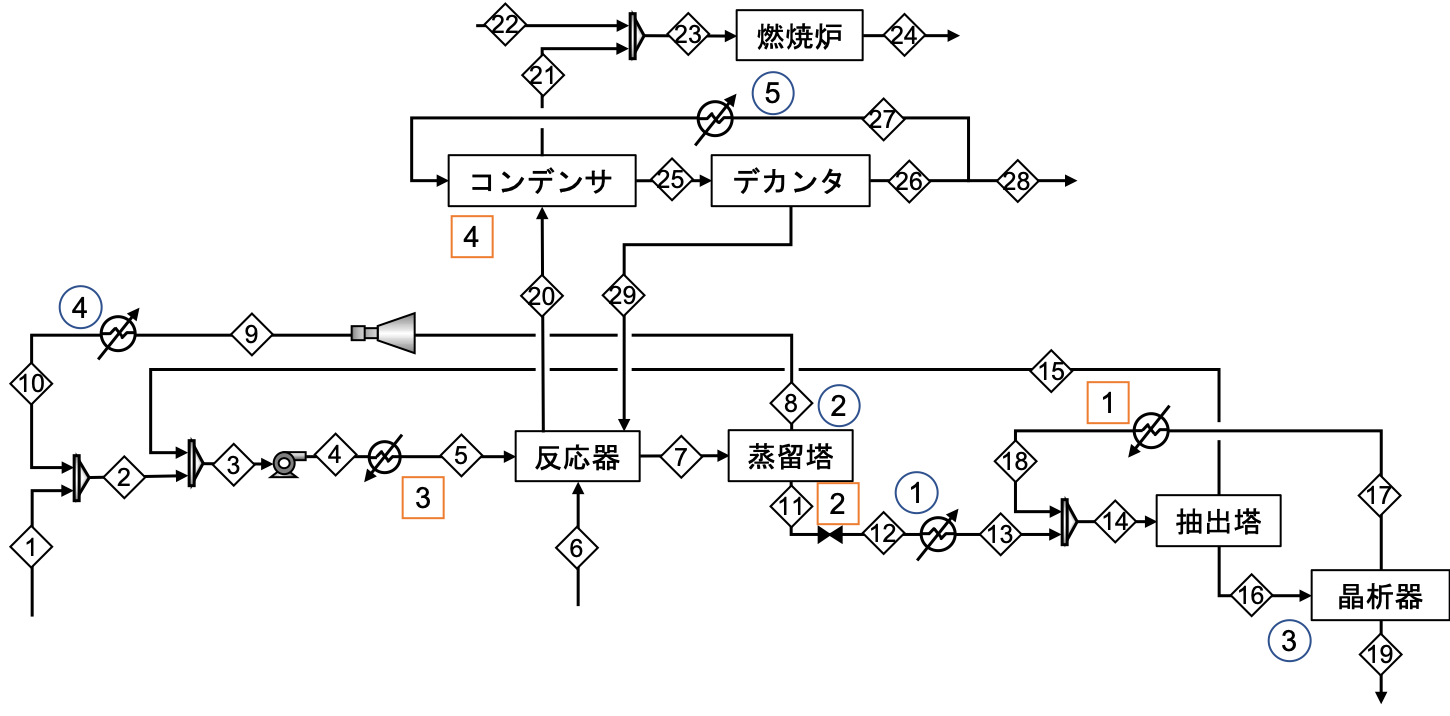
\includegraphics[scale=0.6]{heat_flow.png}
  \caption{与熱流体と受熱流体}
  \label{与熱流体と受熱流体}
\end{figure}

\begin{table}[htbp]
  \centering
  \caption{与熱流体}
  \label{与熱流体}
  \begin{tabular}{lccc}
    \hline
    与熱流体 & 変化前温度 \, [\si{\degreeCelsius}] & 変化後温度 \, [\si{\degreeCelsius}] & 与熱量 \, [\si{\mega \joule \per \hour}] \\
    \hline
    \textcircled{\scriptsize 1} 蒸留塔留出液 & 194.8 & 90.9 & 6338.4 \\
    \textcircled{\scriptsize 2} 蒸留塔コンデンサー & 248.3 & 231.5 & 5111.8 \\
    \textcircled{\scriptsize 3} 晶析器流入流体 & 40.0 & 13.3 & 2252.7 \\
    \textcircled{\scriptsize 4} 蒸留塔缶出液 & 230.9 & 25 & 2436.7 \\
    \textcircled{\scriptsize 5} デカンタ流出純水 & 40.0 & 25 & 1130.6 \\
    \hline
  \end{tabular}
\end{table}

\begin{table}[htbp]
  \centering
  \caption{受熱流体}
  \label{受熱流体}
  \begin{tabular}{lccc}
    \hline
    受熱流体 & 変化前温度 \, [\si{\degreeCelsius}] & 変化後温度 \, [\si{\degreeCelsius}] & 受熱量 \, [\si{\mega \joule \per \hour}] \\
    \hline
    \fbox{\scriptsize 1} 晶析器リサイクル & 13.3 & 40.0 & 2149.3 \\
    \fbox{\scriptsize 2} 蒸留塔リボイラー & 304.0 & 315.6 & 11735.8 \\
    \fbox{\scriptsize 3} 反応器入り口流体 & 76.0 & 170.0 & 2922.4 \\
    \fbox{\scriptsize 4} デカンタ流入純水 & 25.0 & 40.0 & 1130.6 \\
    \hline
  \end{tabular}
\end{table}


\clearpage
\chapter{ヒートインテグレーション}
流体同士の熱交換を行い,外部流体の利用量を削減することを目的としてヒートインテグレーションを行った.
本プロセスにおいては熱交換器は多管型熱交換器として,向流で熱交換を行った.
熱交換面積を求めるため,以下の式を用いた.
\begin{equation}
    Q=UA(\varDelta T)_\mathrm{lm}
\end{equation}
ただし$(\varDelta T)_\mathrm{lm}$は温度差の対数平均であり,熱交換によって与熱流体の温度が$T_\mathrm{h1}$から$T_\mathrm{h2}$に変化し,受熱流体の温度が$T_\mathrm{c2}$から$T_\mathrm{c1}$に変化するとき,
\begin{equation}
    (\varDelta T)_\mathrm{lm} = \frac{(T_\mathrm{h1} - T_\mathrm{c1}) - (T_\mathrm{h2} - T_\mathrm{c2})}{\ln\{(T_\mathrm{h1} - T_\mathrm{c1}) / (T_\mathrm{h2} - T_\mathrm{c2})\}}
\end{equation}
と表される.総括熱伝達係数として,両熱交換流体の相状態にのみ依存するとして表\ref{総括熱伝達係数}の値を用いた.
\begin{table}[htbp]
  \centering
  \caption{総括熱伝達係数}
  \label{総括熱伝達係数}
  \begin{tabular}{ccc}
    \hline
    流体1 & 流体2 & 総括伝熱係数[\si{\watt \per \metre \per \second}] \\
    \hline
    ガス & ガス &150 \\
    ガス & 液 &200 \\
    ガス & ガス(凝縮) & 500 \\
    ガス & 液(蒸発) & 500 \\
    液 & 液 & 300 \\
    液 & ガス(凝縮) & 1000 \\
    液 & 液(蒸発) & 1000 \\
    ガス(凝縮) & 液(蒸発) &1500 \\
    \hline
  \end{tabular}
\end{table}
プロセス内の熱交換流体の温度推移と交換熱量を表に示す.また,用いた外部熱媒の温度と熱量を表に示す.

図\ref{TQ線図}に最終的な設計結果におけるTQ線図を示す.
\begin{figure}[htbp]
  \centering
  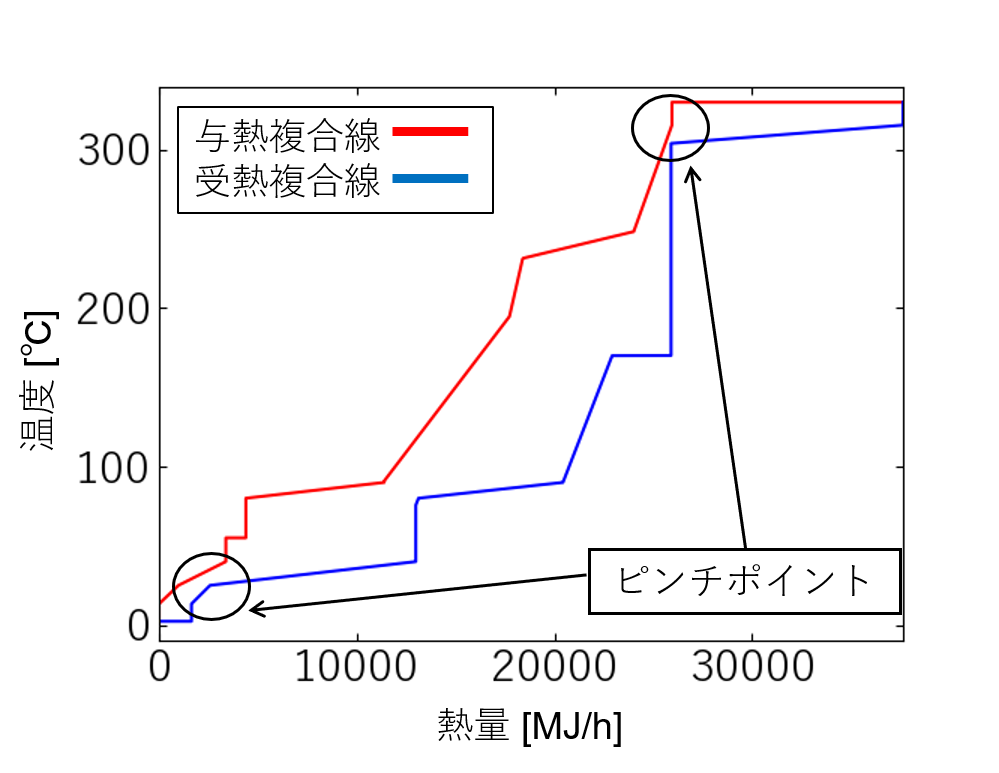
\includegraphics[scale=0.7]{TQdiagram.png}
  \caption{TQ線図}
  \label{TQ線図}
\end{figure}

熱交換により,外部熱媒を用いた場合と比較して,


\clearpage
\chapter{経済評価}
減価償却を8年とした場合の経済評価は表\ref{経済評価}のようになった.なお,各装置費の推算式は,Appendix Aに示した通りである.
\begin{table}[htbp]
    \centering
    \caption{経済評価 [億円/年]}
    \label{経済評価}
    \begin{tabular}{c|c|cc|c}
      \hline
      収入 & 製品 & 安息香酸 & 23.7 & 23.7 \\
      \hline
      \multirow{14}{*}{支出} & 原料コスト & トルエン & 10.4 & 10.4 \\
      \cline{2-5}
      & \multirow{10}{*}{装置コスト} & 晶析器 & 0.39 & \multirow{10}{*}{18.31} \\
      & & 反応器 & 0.34 & \\
      & & 熱交換器 & 0.33 & \\
      & & 抽出塔 & 0.14 & \\
      & & コンデンサ & 0.05 & \\
      & & 燃焼炉 & 0.05 & \\
      & & 蒸留塔 & 0.04 & \\
      & & デカンタ & 0.04 & \\
      & & ポンプ & 0.02 & \\
      & & コンプレッサー & 0.02 & \\
      \cline{2-5}
      & \multirow{3}{*}{運転コスト} & 用役コスト & 1.24 & \multirow{3}{*}{6.60} \\
      & & 触媒 & 0.36 & \\
      & & 人件費 & 5 & \\
      \hline
    \end{tabular}
\end{table}


\clearpage
\chapter{結言}
設計目標を純度99.0 wt\%の安息香酸を年2万ton製造するものとして,設計を行った.
文献値を参考として気液反応器,および晶析装置を設計した.
リサイクルフローを考えて,原料の有効利用を行った.
反応器体積,晶析器体積,晶析器内温度を用いたプロセス全体の3変数同時最適化を行った.
これにより,年 億円の利益を得ると見込める設計となった.

残った課題としては,蒸発トルエンのさらなる回収を行うため,燃焼炉ではなく吸着装置を用いることを検討することや,
各装置についてさらに詳細に設計することが挙げられる.


\clearpage
\chapter*{謝辞}
\addcontentsline{toc}{chapter}{謝辞}
今回のプロセス設計では,様々な方々にお世話になりました.山本教授,谷口准教授を
はじめとする多くの化学工学の先生方,集中講義を実施してくださった玉川先生に感謝の意を申し上げます.

また,1講座の先輩方の協力無しには私たちのプロセス設計は実現できませんでした.
プロセスの内容や発表に対し,的確なアドバイスをいただきました.
お忙しい中,原稿やスライドのチェック,発表練習などに協力して頂いたことで,無事に発表を終えることができました.

私たちのプロセス設計に協力してくださった先生方,先輩方に改めて御礼申し上げます.


\clearpage
\bibliography{bibs/refs.bib}
\begin{thebibliography}{10}
    \bibitem{化工便覧} 化学工学会・化学工学便覧・丸善出版
    \bibitem{晶析} Gary Morris and  Graham Power \textit{et al.  Org. Process Res. Dev.} \textbf{19}, 1891-1902, 2015
    \bibitem{酢酸マンガン} 富士フィルム和光純薬(株) \url{https://labchem-wako.fujifilm.com/jp/product/detail/W01W0113-0065.html}
    \bibitem{モリブデン酸アンモニウム} キシダ化学(株) \url{http://www.kishida.co.jp/product/catalog/detail/id/960}
    \bibitem{プロセスデザインコンテスト10} 化学工学会・SIS部会・情報技術教育分科会, 第10回プロセスデザイン学生コンテスト
    \bibitem{講義資料3} 京都大学・プロセス設計講義資料3
    \bibitem{謎資料} 第6回ソフトウェアツール学生コンテスト \url{http://www.chemeng.titech.ac.jp/~sis_cont/dairokkai.html}
    \bibitem{実験テキスト} 京都大学化学プロセス工学コース 実験テキスト
    \bibitem{TPP} R.Byron Bird and Warren E. Stewart ,Edwin N. Lightfoot   TransPortPhenomena revised second edition   willy
    \bibitem{界面張力}
\end{thebibliography}


\clearpage
\chapter*{変数一覧}
\addcontentsline{toc}{chapter}{変数一覧}
\begin{multicols}{2}
\begin{flushleft}
    $a$:比界面積 \\
    $B^0$:一次核発生速度 \\
    $c$:重量濃度 \\
    $C$:モル濃度 \\
    $C_\mathrm{D}$:抗力係数 \\
    $D$:拡散係数 \\
    $d_\mathrm{vs}$:気泡体積平均径 \\
    $E$:活性化エネルギー \\
    $E_\mathrm{g}$:結晶化過程の活性化エネルギー \\
    $F$:モル流量 \\
    $g$:重力加速度 \\
    $G$:核成長速度 \\
    $k$:反応速度定数 \\
    $k_\mathrm{b}$:核発生速度定数 \\
    $k_\mathrm{g}$:核成長速度定数 \\
    $k_\mathrm{L}$:液相物質移動係数 \\
    $k_\mathrm{L}a$:液相物質移動容量係数 \\
    $k_\mathrm{v}$:結晶体積形状係数 \\
    $M_\mathrm{T}$:懸濁密度 \\
    $n$:結晶の個数密度 \\
    $P_\mathrm{G}$:攪拌動力 \\
    $P_\mathrm{T}$: \\
    $r$:反応速度 \\
    $T$:温度 \\
    $T_\mathrm{c}$:臨界温度 \\
    $u_\mathrm{t}$:気泡の終末速度 \\
    $u_\mathrm{G}$:気泡の空塔速度 \\
    $V$:体積 \\
    $\beta$:還流率 \\
    $\mu$:粘度 \\
    $\mu_\mathrm{L}$:液相粘度 \\
    $\sigma$:界面張力 \\
    $\rho_\mathrm{a}$:空気密度 \\
    $\rho_\mathrm{L}$:液相密度 \\
    $\rho_\mathrm{g}$:気相密度 \\
    $\Delta\rho$:密度差 \\
    $Eo$:エトベス数 \\
    $Sc$:シュミット数 \\
    $Re$:レイノルズ数
\end{flushleft}
\end{multicols}


\appendix
\chapter{コスト推算}
為替レートは1\,ドル=111.73\,円とした.(2019年4月平均)

\section{労務費}
労務費の推算について補足する.プラントは4直3交代で運転され,1班の人数に関して次の推算式を用いた.
\begin{equation}
    (1班の人数) = (6.29 + 0.23 \times (主要機器数))^{0.5}
\end{equation}
よって,総運転員数は40人であり,主任などに10人加え,50人に平均1000\,万円の給与を支払うとして労務費を算出した.

\section{ユーティリティコスト}
用役単価を表\ref{用役単価}に示す.
\begin{table}[htbp]
  \centering
  \caption{用役単価}
  \label{用役単価}
  \begin{tabular}{cc}
    \hline
    項目 & 価格 \\
    \hline
    燃料[\$/ \si{\giga \joule}] & 1.095 \\
    触媒[円/g] & 9.616 \\
    2.3℃プロピレン冷媒[\$/ \si{\giga \joule}] & 4.804 \\
    純水[\$/ \si{\tonne}] & 45 \\
    電力[\$/ \si{\kilo \watt \hour}] & 0.1 \\
    \hline
  \end{tabular}
\end{table}
触媒であるモリブデン酸マンガンは参考文献\cite{Li2019}によると,材料である酢酸マンガン21\,gとモリブデン酸アンモニウム5.04\,gを混ぜて作っている.
各価格について酢酸マンガンは500\,g\,-\,3100\,円とし(\cite{酢酸マンガン},\,2019/7/17確認),モリブデン酸マンガンは500\,g\,-\,11900\,円(\cite{モリブデン酸アンモニウム},\,2019/7/17確認)とした.
燃料,プロピレン冷媒(内挿値)の価格は参考文献\cite{プロセスデザインコンテスト10}より得た.
電力の価格は参考文献\cite{講義資料3}から得た.

さらに\cite{講義資料3}から,排水処理費用としてデカンターからパージする純水に1\,\si{\tonne}あたり0.041\,\$かかるとした.

\section{機器コスト (参考\cite{講義資料3})}
下記の推算は2001年のデータで行い,2001年のコストインデックス394と2018年のコストインデックス603.1を用いて値を修正している.

主要機器について,
\begin{itemize}
    \item[1)]常圧で運転することを想定し,炭素鋼を用いて作成されるとしてメーカー出荷地点での価格を推算
    \item[2)]関連する部分の直接費,間接費を含めた価格の推算
    \item[3)]圧力や材質利用に関する補正
\end{itemize}
という3段階によって機器の建設費を推定する方法を用いた.

まず,メーカー船積み出荷価格$C_\mathrm{p}^0$は,機器の特徴サイズ$A$と係数$K_1, \, K_2, \, K_3$を用いて
\begin{equation}
    \log_{10}C_\mathrm{p}^0 = K_1 + K_2\log_{10} A + K_3(\log_{10} A)^2
\end{equation}

直接費や間接費,特殊材料費,操作圧力を考慮すると,各装置に関係するコストは$C_\mathrm{p}^0$の数倍になる.
すなわち,
\begin{equation}
    C_\mathrm{BM} = F_\mathrm{BM} C_\mathrm{p}^0
\end{equation}
と表される.$C_\mathrm{BM}, \, F_\mathrm{BM}$はそれぞれベアモジュールコスト,ベアモジュールファクターと呼ばれる.
$F_\mathrm{BM}$は,
\begin{equation}
    F_\mathrm{BM} = B_1 + B_2 F_\mathrm{p} F_\mathrm{M}
\end{equation}
と表される.ここで,$B_1, \, B_2, \, F_\mathrm{p}, \, F_\mathrm{M}$はそれぞれ圧力,材質に依存しない部分の係数,依存する部分の係数,圧力ファクター,材質ファクターを表す.
$F_\mathrm{p}$に関しては槽型の装置に対して推算式\eqref{槽型推算式}が提示されている.
\begin{center}
\begin{equation}
    F_\mathrm{p,vessel} =
        \begin{dcases}
            \max \left\{\dfrac{(P_\mathrm{g} + 1 )D}{10.71 - 0.00756(P_\mathrm{g} + 1)}+0.5 \, , \, 1 \right\} & (P_\mathrm{g} > -0.5\, \si{\bar}) \\
            1.25 & (P_\mathrm{g} \leq -0.5\, \si{\bar})
        \end{dcases}
    \label{槽型推算式}
\end{equation}
\end{center}
ただし,$P_\mathrm{g}$はゲージ圧\si{[\bar]}である.槽型以外の装置については,次式を用いた.
\begin{equation}
    \log_{10}F_\mathrm{p} = C_1 + C_2\log_{10} P_\mathrm{g} + C_3(\log_{10} P_\mathrm{g})^2
\end{equation}

各機器のコスト算出に当たって用いた係数を表\ref{BM係数}に示す.
\begin{table}[htbp]
  \centering
  \caption{ベアモジュールファクター算出に用いた係数}
  \label{BM係数}
  \scalebox{0.9}{
  \begin{tabular}{cccccccccccc}
  \hline
  & $A$ & $K_1$ & $K_2$ & $K_3$ & $B_1$ & $B_2$ & $C_1$ & $C_2$ & $C_3$ & 材質 & $F_\mathrm{M}$  \\
  \hline
  反応器 & 体積[\si{\cubic\metre}] & 4.5587 & 0.2986 & 0.002  & 1.49 & 1.52 & - & - & - & Ti clad & 4.8 \\
  晶析器 & 体積[\si{\cubic\metre}] & 4.5097 & 0.1781 & 0.1344 & 1.49 & 1.52 & - & - & - & Ti alloy clad & 9.4 \\
  蒸留塔(槽) & 体積[\si{\cubic\metre}] & 3.4974 & 0.4485 & 0.1074 & 1.49 & 1.52 & - & - & - & Ti clad & 4.8 \\
  蒸留塔(トレイ)& 面積[\si{\square\metre}] & 2.9949 & 0.4465 & 0.3961 & 1.49 & 1.52 & - & - & - & Ti clad & 4.8 \\
  抽出塔 & 体積[\si{\cubic\metre}] & 3.4974 & 0.4485 & 0.1074 & 1.49 & 1.52 & - & - & - & Ti & 9.4 \\
  デカンター & 体積[\si{\cubic\metre}] & 3.4974 & 0.4485 & 0.1074 & 2.25 & 1.82 & - & -& - & CC & 1 \\
  燃焼炉 & 燃焼熱量[\si{\kilo \watt}] & 3.068  & 0.6597 & 0.0194 & - & - & 0 & 0& 0 &  CC & 1 \\
  ポンプ & 電力[\si{\kilo\watt}] & 3.8696 & 0.3161 & 0.122  & 1.89 & 1.35 & 0 & 0& 0 & Ni alloy & 3.9 \\
  コンプレッサー& 電力[\si{\kilo\watt}] & 2.2897 & 1.3604 & -0.103 & - & - & 0 & 0 & 0 & CC & 1  \\
  \hline
  \end{tabular}
  }
\end{table}
データが資料にない機器についてはベアモジュールファクターを1とした.

熱交換器については,伝熱面積を$A \, [\si{\square\metre}]$として次の計算式を用いた\cite{謎資料}.
\begin{equation}
    \text{(コスト [億円])} = 0.015K \times A^{0.65}
\end{equation}
ただし,$K$は定数でありコンデンサーは1,リボイラーは2とした.

\end{document}
